\documentclass[aspectratio=169]{beamer}
\usetheme{Madrid}
\usecolortheme{dolphin}
\usepackage[utf8]{inputenc}
\usepackage[T1]{fontenc}
\usepackage[french]{babel}
\usepackage{lmodern}
\usepackage{hyperref}
\usepackage{booktabs}
\usepackage{tikz}
\usepackage{xcolor}
\usepackage{colortbl}

\title{IA pour la théorie}
\subtitle{État de l'art, usages et actions pour la communauté}
\author{Gabriel Peyré \\ CNRS et ENS, Université PSL}
\date{2 juillet 2026}

\definecolor{aiNavy}{HTML}{26364F}
\definecolor{aiBlue}{HTML}{2F6FA3}
\definecolor{aiTeal}{HTML}{238C82}
\definecolor{aiGreen}{HTML}{3F8A5F}
\definecolor{aiAmber}{HTML}{B7791F}
\definecolor{aiRed}{HTML}{A84E4E}
\definecolor{aiViolet}{HTML}{6C63C7}
\definecolor{aiSlate}{HTML}{6D7480}
\definecolor{softBlue}{HTML}{EAF2FB}
\definecolor{softTeal}{HTML}{E6F5F2}
\definecolor{softGreen}{HTML}{ECF7EE}
\definecolor{softAmber}{HTML}{FFF2D7}
\definecolor{softRed}{HTML}{FBEDED}
\definecolor{softViolet}{HTML}{F0EEFB}
\definecolor{softGray}{HTML}{F4F6F8}
\definecolor{softGrayA}{HTML}{F7F8FA}
\definecolor{softGrayB}{HTML}{F1F4F7}
\definecolor{softGrayC}{HTML}{ECEFF3}
\definecolor{softGrayD}{HTML}{F5F5F2}
\definecolor{softGrayE}{HTML}{F0F2F4}

\setbeamercolor{structure}{fg=aiBlue}
\setbeamercolor{title}{fg=aiNavy}
\setbeamercolor{subtitle}{fg=aiBlue}
\setbeamercolor{frametitle}{fg=aiNavy,bg=softBlue}
\setbeamerfont{frametitle}{series=\bfseries}
\setbeamercolor{palette primary}{fg=white,bg=aiNavy}
\setbeamercolor{palette secondary}{fg=white,bg=aiBlue}
\setbeamercolor{palette tertiary}{fg=white,bg=aiTeal}
\setbeamercolor{palette quaternary}{fg=white,bg=aiViolet}
\setbeamercolor{box claim}{fg=black,bg=softGrayA}
\setbeamercolor{box proof}{fg=black,bg=softGrayB}
\setbeamercolor{box example}{fg=black,bg=softGrayC}
\setbeamercolor{box action}{fg=black,bg=softGrayD}
\setbeamercolor{box risk}{fg=black,bg=softGrayE}
\setbeamercolor{box danger}{fg=black,bg=softGrayC}
\setbeamercolor{box neutral}{fg=black,bg=softGrayA}
\setbeamercolor{box neutral alt}{fg=black,bg=softGrayC}
\setbeamercolor{box problem}{fg=black,bg=softBlue}
\setbeamercolor{box result}{fg=black,bg=softTeal}
\setbeamercolor{box takeaway}{fg=black,bg=softAmber}
\setbeamertemplate{itemize item}{\raise0.15ex\hbox{\scriptsize\color{aiBlue}\(\blacktriangleright\)}}
\setbeamertemplate{itemize subitem}{\raise0.15ex\hbox{\tiny\color{aiTeal}\(\blacktriangleright\)}}
\setbeamertemplate{blocks}[rounded][shadow=false]

\newcommand{\source}[1]{\vspace{1mm}{\tiny\color{aiSlate}Source : #1}}
\newenvironment{claimbox}{\begin{beamercolorbox}[wd=\linewidth,rounded=true,sep=1.1mm]{box claim}}{\end{beamercolorbox}}
\newenvironment{proofbox}{\begin{beamercolorbox}[wd=\linewidth,rounded=true,sep=1.1mm]{box proof}}{\end{beamercolorbox}}
\newenvironment{examplebox}{\begin{beamercolorbox}[wd=\linewidth,rounded=true,sep=1.1mm]{box example}}{\end{beamercolorbox}}
\newenvironment{actionbox}{\begin{beamercolorbox}[wd=\linewidth,rounded=true,sep=1.1mm]{box action}}{\end{beamercolorbox}}
\newenvironment{riskbox}{\begin{beamercolorbox}[wd=\linewidth,rounded=true,sep=1.1mm]{box risk}}{\end{beamercolorbox}}
\newenvironment{dangerbox}{\begin{beamercolorbox}[wd=\linewidth,rounded=true,sep=1.1mm]{box danger}}{\end{beamercolorbox}}
\newenvironment{neutralbox}{\begin{beamercolorbox}[wd=\linewidth,rounded=true,sep=1.1mm]{box neutral}}{\end{beamercolorbox}}
\newenvironment{neutralboxalt}{\begin{beamercolorbox}[wd=\linewidth,rounded=true,sep=1.1mm]{box neutral alt}}{\end{beamercolorbox}}
\newenvironment{problembox}{\begin{beamercolorbox}[wd=\linewidth,rounded=true,sep=1.0mm]{box problem}}{\end{beamercolorbox}}
\newenvironment{resultbox}{\begin{beamercolorbox}[wd=\linewidth,rounded=true,sep=1.0mm]{box result}}{\end{beamercolorbox}}
\newenvironment{takeawaybox}{\begin{beamercolorbox}[wd=\linewidth,rounded=true,sep=1.0mm]{box takeaway}}{\end{beamercolorbox}}
\newcommand{\problemlabel}{\textbf{\textcolor{aiBlue}{Problème}}}
\newcommand{\resultlabel}{\textbf{\textcolor{aiTeal}{Résultats}}}
\newcommand{\takeawaylabel}{\textbf{\textcolor{aiAmber}{Takeaway}}}
\newlength{\keylabelwidth}
\newcommand{\keyitem}[2]{%
  \item \settowidth{\keylabelwidth}{\textbf{#1} : }%
  \makebox[\keylabelwidth][l]{\textbf{#1} : }%
  \parbox[t]{\dimexpr\linewidth-\keylabelwidth-0.6em\relax}{\raggedright #2}%
}
\newcommand{\keyline}[2]{%
  \settowidth{\keylabelwidth}{\textbf{#1} : }%
  \noindent\makebox[\keylabelwidth][l]{\textbf{#1} : }%
  \parbox[t]{\dimexpr\linewidth-\keylabelwidth-0.6em\relax}{\raggedright #2}\par%
}
\newcommand{\labelline}[2]{%
  \settowidth{\keylabelwidth}{#1 : }%
  \noindent\makebox[\keylabelwidth][l]{#1 : }%
  \parbox[t]{\dimexpr\linewidth-\keylabelwidth-0.6em\relax}{\raggedright #2}\par%
}
\newcommand{\plantile}[7]{%
  \begin{scope}[shift={(#1,#2)},opacity=#7]
    \filldraw[fill=#5,draw=aiSlate!38,line width=0.65pt,rounded corners=2.5pt] (0,0) rectangle (5.72,2.62);
    \draw[#6!60,line width=1.0pt] (0.20,0.28) -- (0.20,2.36);
    \node[anchor=north west,font=\bfseries\large,text=black,inner sep=0pt,align=left,text width=5.15cm] at (0.38,2.38) {#3};
    \begin{scope}
      \clip[rounded corners=1.5pt] (0.30,0.24) rectangle (5.42,1.56);
      \node[inner sep=0pt] at (2.86,0.90) {\includegraphics[width=5.12cm,height=1.32cm,keepaspectratio]{#4}};
    \end{scope}
  \end{scope}
}
\newcommand{\planslide}[1]{%
\ifnum#1=1\def\planopone{1}\else\def\planopone{0.34}\fi
\ifnum#1=2\def\planoptwo{1}\else\def\planoptwo{0.34}\fi
\ifnum#1=3\def\planopthree{1}\else\def\planopthree{0.34}\fi
\ifnum#1=4\def\planopfour{1}\else\def\planopfour{0.34}\fi
\begin{frame}{Plan de l'exposé}
\vspace{-1mm}
\begin{center}
\begin{tikzpicture}[x=1cm,y=1cm]
  \plantile{0}{3.02}{LLMs et maths}{assets/generated/imo_2025_problem1_crop.png}{softGrayA}{aiBlue}{\planopone}
  \plantile{6.02}{3.02}{IA pour la recherche\\en maths}{assets/generated/unit_distance_series.png}{softGrayB}{aiTeal}{\planoptwo}
  \plantile{0}{0.12}{Retours d'expérience}{assets/generated/noogram_flow_matching_site.png}{softGrayD}{aiAmber}{\planopthree}
  \plantile{6.02}{0.12}{Impact sur la\\communauté}{assets/generated/paperreview_ai_screenshot.png}{softGrayC}{aiViolet}{\planopfour}
\end{tikzpicture}
\end{center}
\end{frame}
}

\begin{document}

\begin{frame}[plain]
\centering
\vspace{1.25cm}
{\fontsize{34}{40}\selectfont\bfseries\textcolor{aiNavy}{IA pour la théorie}\par}
\vspace{0.45cm}
{\Large\textcolor{aiBlue}{État de l'art, usages et actions pour la communauté}\par}
\vspace{0.9cm}
{\large Gabriel Peyré\par}
\vspace{0.15cm}
{\normalsize\textcolor{aiSlate}{CNRS et ENS, Université PSL}\par}
\vfill
{\small\textcolor{aiSlate}{2 juillet 2026}\par}
\vspace{0.18cm}
{\scriptsize\href{https://github.com/gpeyre/ia4maths}{\textcolor{aiBlue}{\texttt{github.com/gpeyre/ia4maths}}}\par}
\end{frame}

\planslide{1}

\begin{frame}{IA pour les maths}
\small
\begin{columns}[T,totalwidth=\linewidth]
\column{0.49\linewidth}
\begin{actionbox}
\textbf{IA pour la découverte scientifique}\par
\vspace{1mm}
{\centering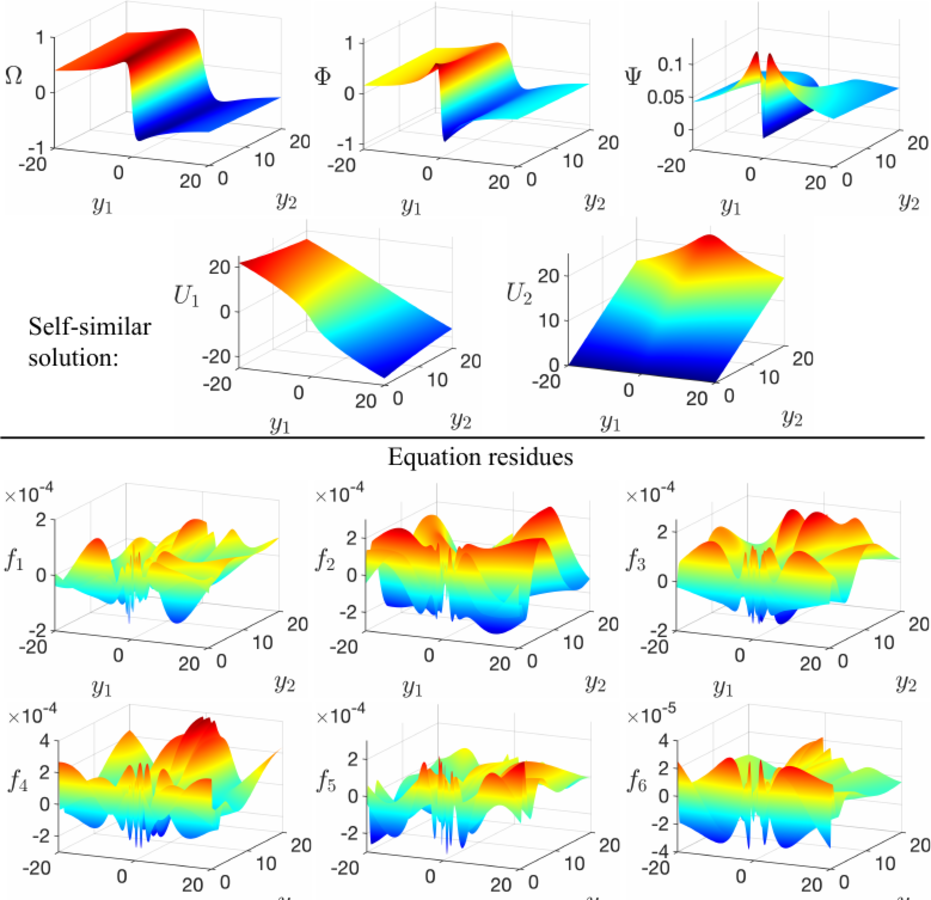
\includegraphics[height=0.34\textheight,keepaspectratio]{assets/generated/euler_pinn_blowup_crop.png}\par}
\vspace{0.5mm}
\raggedright{\scriptsize PINNs pour explorer des EDP : Navier--Stokes / Euler, instabilités, contre-exemples.}
\end{actionbox}

\column{0.49\linewidth}
\begin{proofbox}
\textbf{IA pour la preuve de théorèmes}\par
\vspace{1mm}
{\centering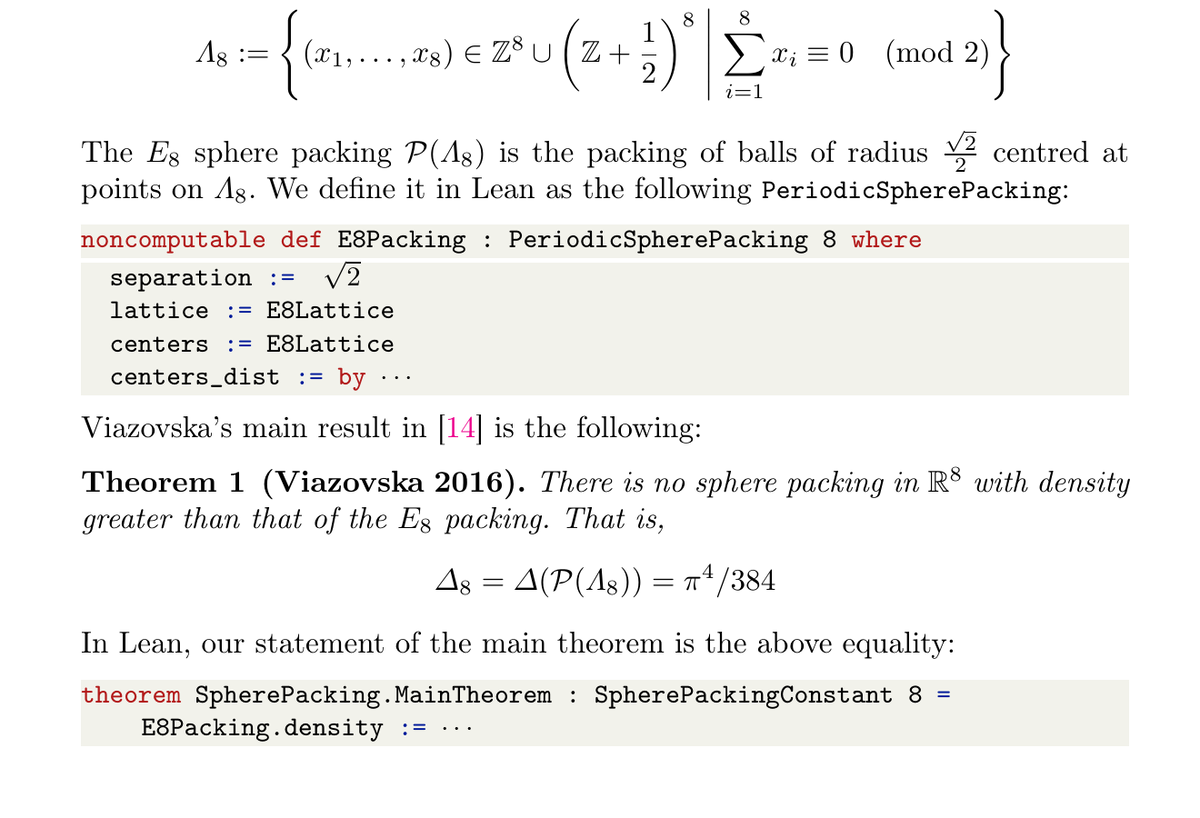
\includegraphics[height=0.32\textheight,keepaspectratio]{assets/generated/sphere_packing_lean_crop.png}\par}
\vspace{0.5mm}
\raggedright{\scriptsize Lean : preuve vérifiée ; Viazovska, empilement optimal de \(E_8\).}
\end{proofbox}
\end{columns}

\vspace{1mm}
\begin{claimbox}
\textbf{Focus} : raisonnement mathématique, de l'informel au formel.
\end{claimbox}
\source{Wang--Lai--Gómez-Serrano--Buckmaster, arXiv:2201.06780 ; Hariharan et al., arXiv:2604.23468.}
\end{frame}

\begin{frame}{LLMs pour le raisonnement et les maths}
\small
\begin{center}
\begin{tikzpicture}[x=1.02cm,y=1cm]
  \tikzset{
    foundation/.style={font=\scriptsize,align=center,text width=1.55cm,inner sep=2.3pt,draw=aiSlate!35,fill=softGrayA,rounded corners=1.5pt},
    tag/.style={font=\scriptsize,anchor=west}
  }
  \draw[->,thick,aiNavy] (0,0) -- (10.2,0);
  \foreach \x/\y in {0/2017,1.45/2020,3.05/2022,4.55/2024,6.05/2025,7.75/2025,9.65/2026}
    {\draw[aiNavy] (\x,0.08) -- (\x,-0.08) node[below=3pt,text=aiSlate] {\scriptsize \y};}

  \node[foundation,anchor=south] at (0.15,0.28)
    {\textbf{Transformer}\\architecture};
  \node[foundation,fill=softGrayB,anchor=south] at (1.45,1.13)
    {\textbf{GPT-3}\\échelle};
  \node[foundation,fill=softGrayD,anchor=south] at (3.05,0.28)
    {\textbf{ChatGPT}\\usage massif};

  \filldraw[draw=aiSlate!40,fill=softGrayB,rounded corners=1.5pt] (4.25,0.80) rectangle (10.15,2.02);
  \node[tag] at (4.40,1.80) {\textbf{Raisonnement}};
  \node[tag] at (4.40,1.48) {\textbf{o1/o3}};
  \node[tag] at (5.55,1.48) {\textbf{DeepSeek-R1}};
  \node[tag] at (7.35,1.48) {\textbf{Gemini Deep Think}};
  \node[tag] at (4.40,1.12) {\textbf{Claude reasoning}};

  \filldraw[draw=aiSlate!40,fill=softGrayC,rounded corners=1.5pt] (4.25,-2.05) rectangle (10.15,-0.70);
  \node[tag] at (4.40,-0.94) {\textbf{Agentique / code}};
  \node[tag] at (4.40,-1.27) {\textbf{Codex}};
  \node[tag] at (5.55,-1.27) {\textbf{Claude Code}};
  \node[tag] at (7.35,-1.27) {\textbf{Mistral vibe}};
  \node[tag] at (4.40,-1.63) {\textbf{OpenClaws}};
\end{tikzpicture}
\end{center}
\end{frame}

\begin{frame}{Pourquoi les maths sont devenues centrales pour les LLMs}
\small
\begin{problembox}
\problemlabel{} : les maths comme banc d'essai du raisonnement.
\end{problembox}
\vspace{1mm}
\begin{itemize}
  \keyitem{Entraînement}{\textit{next-token prediction}, évaluation orientée \textcolor{aiTeal}{raisonnement}.}
  \keyitem{Benchmarks}{GSM8K, MATH, AIME/IMO-style comme signaux stratégiques.}
  \keyitem{Raisonnement}{\textit{reinforcement learning} et récompenses mathématiques.}
\end{itemize}
\vspace{1mm}
\begin{examplebox}
\scriptsize
\textbf{Snippets de benchmark}
\vspace{0.2mm}

\setlength{\tabcolsep}{4pt}
\begin{tabular}{@{}p{0.18\linewidth}p{0.76\linewidth}@{}}
\textbf{GSM8K} & arithmétique verbale : \textit{``Alice achète 3 carnets... combien reste-t-il ?''} \\
\textbf{MATH} & problème concours : algèbre / géométrie / analyse, solution structurée. \\
\textbf{AIME / IMO} & énoncé court, recherche longue : déterminer, optimiser, prouver.
\end{tabular}
\end{examplebox}
\vspace{1mm}
\begin{takeawaybox}
\takeawaylabel{} : IA agentique : du local au pipeline complet -- planifier, coder, vérifier, rédiger.
\end{takeawaybox}
\source{Cobbe et al. 2021; Hendrycks et al. 2021; OpenAI Codex 2025/2026.}
\end{frame}

\begin{frame}{Problèmes simples: Olympiade de maths}
\begin{columns}[T,totalwidth=\linewidth]
\column{0.49\textwidth}
\small
\begin{resultbox}
\resultlabel{} 2024 : raisonnement formel\\
AlphaProof + AlphaGeometry 2, traduction en langages formels puis preuve : \textbf{28/42}.
\end{resultbox}

\column{0.49\textwidth}
\begin{resultbox}
\resultlabel{} 2025 : raisonnement informel\\
Gemini Deep Think, modèles génériques et preuves informelles : \textbf{35/42}.
\end{resultbox}
\end{columns}
\vspace{1mm}
\begin{examplebox}
{\scriptsize\textbf{Énoncé officiel IMO 2025}}
\vspace{0.5mm}

\centering
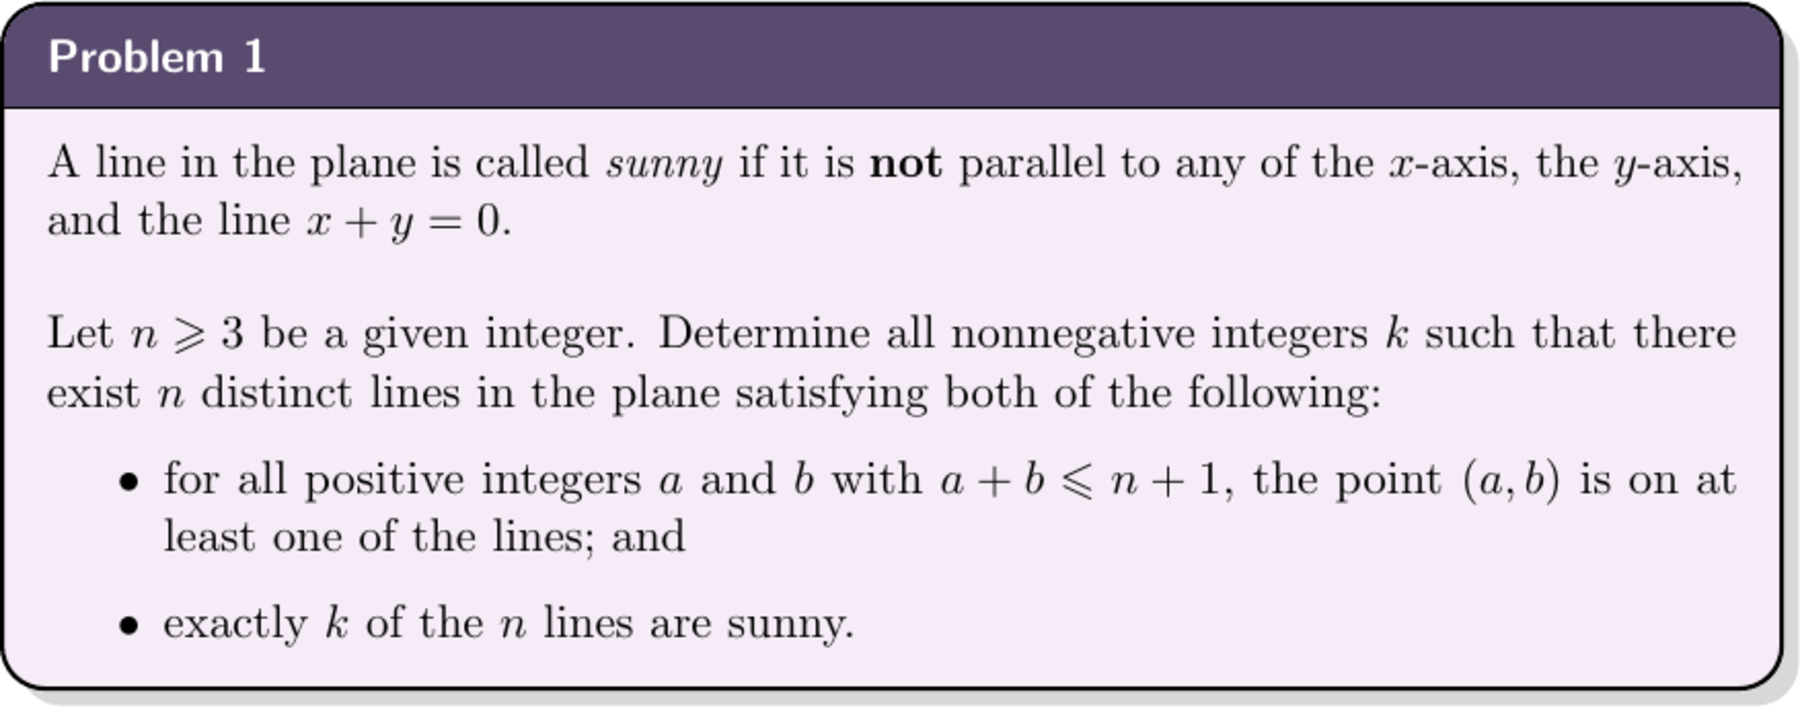
\includegraphics[width=0.98\linewidth,height=0.38\textheight,keepaspectratio]{assets/generated/imo_2025_problem1_crop.png}
\end{examplebox}
\vspace{-0.5mm}
\source{DeepMind 25/07/2024 et 21/07/2025; PDF officiel IMO 2025 (Deep Think).}
\end{frame}

\planslide{2}

\begin{frame}{Niveau recherche : First Proof, du pilote au benchmark}
\footnotesize
\begin{problembox}
\labelline{\problemlabel{}}{mesurer de façon reproductible la preuve de recherche.}
\vspace{-0.3mm}
\scriptsize \keyline{Tâche}{problèmes inédits, solutions humaines disponibles, rédaction complète ; \textbf{critère} : acceptation après revue anonymisée.}
\end{problembox}

\vspace{0.8mm}
\begin{resultbox}
\resultlabel{} : First Batch \(\rightarrow\) Second Batch
\vspace{0.1mm}

\begin{columns}[T,totalwidth=\linewidth]
\column{0.48\linewidth}
\scriptsize
\textbf{\textcolor{aiTeal}{First Batch (02/2026)}}\\[-0.3mm]
\keyline{Signal}{\(\sim\)\textbf{2} succès nets (Q9,Q10).}
\vspace{-0.7mm}
\keyline{Zone grise}{Q5/Q8 proches ou réparables ; pas de revue formelle.}

\column{0.50\linewidth}
\scriptsize
\textbf{\textcolor{aiTeal}{Second Batch (03--06/2026)}}\\[-0.3mm]
\keyline{OK}{\textbf{17/39} soumissions acceptées.}
\vspace{-0.7mm}
\keyline{Couverture}{\textbf{7/10} problèmes avec \(\geq 1\) solution OK.}
\vspace{-0.7mm}
\keyline{Critère}{flawless ou minor revisions après revue experte anonymisée.}
\end{columns}
\end{resultbox}

\vspace{0.8mm}
\begin{takeawaybox}
\scriptsize
\takeawaylabel{} : changement d'échelle, mais validation humaine toujours centrale.
\begin{itemize}
\itemsep0mm
  \keyitem{Capacité}{preuves sérieuses possibles sur problèmes non triviaux.}
  \keyitem{Coûts}{2e batch, \$117--\$4.8k pour les 10 réponses ; \(\sim\)\$10--\$480/réponse.}
  \keyitem{Goulet}{revue experte, lemmes sautés, ``arguments standards'', citations fragiles.}
  \keyitem{Benchmark}{prompts, logs, tokens, temps, coûts et critères d'acceptation.}
\end{itemize}
\end{takeawaybox}

\vspace{0.2mm}
{\tiny\color{aiSlate}Source : ressources/first-proof-summary.md ; \href{https://1stproof.org/}{1stProof} ; arXiv:2602.05192 ; arXiv:2606.18119.}
\end{frame}

\begin{frame}{Niveau recherche : unit distance conjecture}
\begin{columns}[T]
\column{0.47\textwidth}
\scriptsize
\begin{problembox}
\labelline{\problemlabel{}}{\(u(n)\), maximum de paires à distance \(1\) parmi \(n\) points du plan.}
\end{problembox}

\vspace{-0.2mm}
\begin{examplebox}
{\scriptsize\textbf{Prompt OpenAI (résumé)}}\\[-0.5mm]
\tiny
\textit{``Resolve Erd\H{o}s's planar unit-distance problem completely.''}\\[-0.2mm]
Prouver soit \(u(n)\le n^{1+O(1/\log\log n)}\), soit des contre-exemples à toute borne
\(n^{1+C/\log\log n}\). \textbf{Pas de progrès partiel.}
\end{examplebox}

\vspace{-0.2mm}
\begin{resultbox}
\labelline{\resultlabel{}}{contre-exemple OpenAI, puis vérification et optimisation humaines.}
\vspace{-0.8mm}
{\centering\scriptsize \(1+o(1)\quad\leadsto\quad\mathbf{1.0152}\)\par}
\vspace{-0.8mm}
{\centering\tiny
\setlength{\tabcolsep}{3pt}
\renewcommand{\arraystretch}{0.84}
\begin{tabular}{@{}lcccc@{}}
\toprule
& Class. & OpenAI & Sawin & Emmerich \\
\midrule
\rowcolor{softTeal}
Exp. & \(1+o(1)\) & \(>1\) & \(1.014\) & \(\mathbf{1.0152}\) \\
\bottomrule
\end{tabular}
\par
}
\end{resultbox}

\vspace{-0.2mm}
\begin{takeawaybox}
\tiny
\labelline{\takeawaylabel{}}{LLM + harness \(\Rightarrow\) niveau étudiant en thèse sur question ouverte.}
\end{takeawaybox}

\column{0.52\textwidth}
\centering

\includegraphics[width=\linewidth,height=0.70\textheight,keepaspectratio]{assets/generated/unit_distance_series.pdf}

\vspace{-1mm}
{\tiny\color{aiSlate}\raggedright Sources : OpenAI, preuve PDF p.3 ; Alon et al. 2605.20695 ; Sawin 2605.20579 ; Emmerich 2606.03419.\par}
\end{columns}
\end{frame}

\begin{frame}{Maths formelles : théorème de Viazovska (Lean)}
\footnotesize
\begin{problembox}
\problemlabel{} : formaliser un résultat existant majeur.
\begin{itemize}
\itemsep0mm
  \keyitem{Objet}{empilement optimal en dimension \(8\) (Viazovska), extension en dimension \(24\).}
  \keyitem{Enjeu}{transférer une preuve de très haut niveau dans Lean.}
\end{itemize}
\end{problembox}

\vspace{0.6mm}
\begin{resultbox}
\resultlabel{} : dépôt public Math, Inc. \texttt{Sphere-Packing-Lean}.
\begin{itemize}
\itemsep0mm
  \keyitem{Statut}{projet Lean public, massif, centré sur la certification de l'empilement \(E_8\) / Leech.}
  \keyitem{Portée}{géométrie des nombres, théorie du codage, médaille Fields 2022.}
  \keyitem{Taille actuelle}{\textbf{830 fichiers}, \textbf{180\,661 lignes Lean} ; référence FLT Lean : \textbf{117 fichiers}, \textbf{15\,411 lignes}.}
\end{itemize}
\end{resultbox}

\vspace{0.6mm}
\begin{takeawaybox}
\scriptsize
\takeawaylabel{} : certification formelle à grande échelle, mais gouvernance sensible.
\begin{itemize}
\itemsep0mm
  \keyitem{Point de gouvernance}{transfert académique (EPFL) \(\rightarrow\) privé (Math, Inc.) très controversé.}
  \keyitem{Tension}{crédit scientifique, maintenance du code, infrastructure Lean ouverte.}
\end{itemize}
\end{takeawaybox}
\source{Dépôts GitHub ; Hariharan et al., arXiv:2604.23468 ; comptage local 09/03/2026 via \texttt{rg} + \texttt{wc -l}.}
\end{frame}

\begin{frame}{Maths formelles : analyse / EDP (Lean)}
\footnotesize
\begin{problembox}
\labelline{\problemlabel{}}{formaliser l'analyse moderne, encore peu couverte par \texttt{mathlib}.}
\vspace{-0.3mm}
\scriptsize Cas d'usage standard : expert maths non spécialiste Lean, guidé par LLM + vérification formelle.
\end{problembox}

\vspace{0.8mm}
\begin{columns}[T,totalwidth=\linewidth]
\column{0.58\linewidth}
\begin{resultbox}
\labelline{\resultlabel{}}{\textbf{Scott Armstrong} (EDP) et Julia Kempe ; Harnack, Hölder et bases d'analyse réutilisables dans \texttt{scottnarmstrong/DeGiorgi}.}
\vspace{-0.4mm}
{\scriptsize\textbf{Extrait abrégé : \texttt{Harnack.lean}}}\\[-0.7mm]
\begin{beamercolorbox}[wd=\linewidth,rounded=true,sep=0.6mm]{box neutral}
\tiny\ttfamily
\textcolor{aiTeal}{theorem} harnack\\
\quad (A : NormalizedEllipticCoeff d (ball 0 1))\\
\quad (hsol : IsSolution A.1 u) :\\
\quad essSup u \(\mu_{1/2}\) \(\le\)
 exp(C\_harnack d * A.1.\(\Lambda^{1/2}\)) * essInf u \(\mu_{1/2}\) := by ...
\end{beamercolorbox}

\vspace{0.6mm}
\centering
\begin{tikzpicture}[x=1cm,y=1cm]
  \node[draw=aiTeal,fill=softTeal,rounded corners=1pt,inner sep=2pt] (s) at (0,0) {\tiny Sobolev};
  \node[draw=aiTeal,fill=softTeal,rounded corners=1pt,inner sep=2pt] (w) at (1.45,0) {\tiny Harnack faible};
  \node[draw=aiTeal,fill=softTeal,rounded corners=1pt,inner sep=2pt] (h) at (3.25,0) {\tiny Harnack};
  \node[draw=aiTeal,fill=softTeal,rounded corners=1pt,inner sep=2pt] (r) at (4.55,0) {\tiny Hölder};
  \draw[->,aiTeal] (s) -- (w);
  \draw[->,aiTeal] (w) -- (h);
  \draw[->,aiTeal] (h) -- (r);
\end{tikzpicture}
\end{resultbox}

\column{0.40\linewidth}
\begin{takeawaybox}
\takeawaylabel{}\\[-0.5mm]
\tiny
\begin{itemize}
\itemsep0mm
  \keyitem{Faisabilité}{analyse moderne avec Claude/Codex pro.}
  \keyitem{Expertise}{guidage maths indispensable ; hors domaine impossible.}
  \keyitem{Coût}{beaucoup de tokens, supportable si blueprint solide.}
  \keyitem{Tension}{expert maths vs idiome Lean / core dev.}
  \keyitem{Objectif}{bases formalisées pour mettre Lean dans la boucle.}
\end{itemize}
\end{takeawaybox}
\end{columns}
\vspace{0mm}
{\tiny\color{aiSlate}Source : Armstrong--Kempe, arXiv:2604.05984 ; \texttt{scottnarmstrong/DeGiorgi}, notamment \texttt{Harnack.lean} ; billet Armstrong 07/04/2026.}
\end{frame}

\planslide{3}

\begin{frame}{Mon retour d'expérience (recherche)}
\begin{columns}[T]
\column{0.58\textwidth}
\scriptsize
\begin{problembox}
\labelline{\problemlabel{}}{avancer sur un problème assez bien circonscrit où l'on bloque ; faire du Lean en non spécialiste.}
\end{problembox}

\vspace{0.5mm}
\begin{resultbox}
\resultlabel{} : retour personnel sur un usage intensif.
\begin{itemize}
\itemsep0mm
  \keyitem{Déblocage}{problème ouvert résolu en \textbf{2 semaines} via prompts GPT-5 intensifs.}
  \keyitem{Prépublication}{\url{https://arxiv.org/abs/2602.01372}}
  \keyitem{Agents}{Codex / Claude Code en usage quotidien.}
  \keyitem{Bibliothèque}{\url{https://github.com/gpeyre/flow-sinkhorn}}
\end{itemize}
\end{resultbox}

\vspace{0.5mm}
\begin{takeawaybox}
\tiny
\takeawaylabel{} : deux régimes et gains de workflow.
\begin{itemize}
\itemsep0mm
  \keyitem{Informel}{débloque des problèmes ouverts.}
  \keyitem{Formel (Lean)}{fonctionne, mais coûte \(\sim 10\times\) plus de tokens.}
  \keyitem{Rédaction}{prototypage plus rapide.}
  \keyitem{Technique}{tâches répétitives automatisées.}
  \keyitem{Raisonnement}{Lean certifie, mais n'invente pas l'idée.}
\end{itemize}
\end{takeawaybox}
\column{0.42\textwidth}
\centering
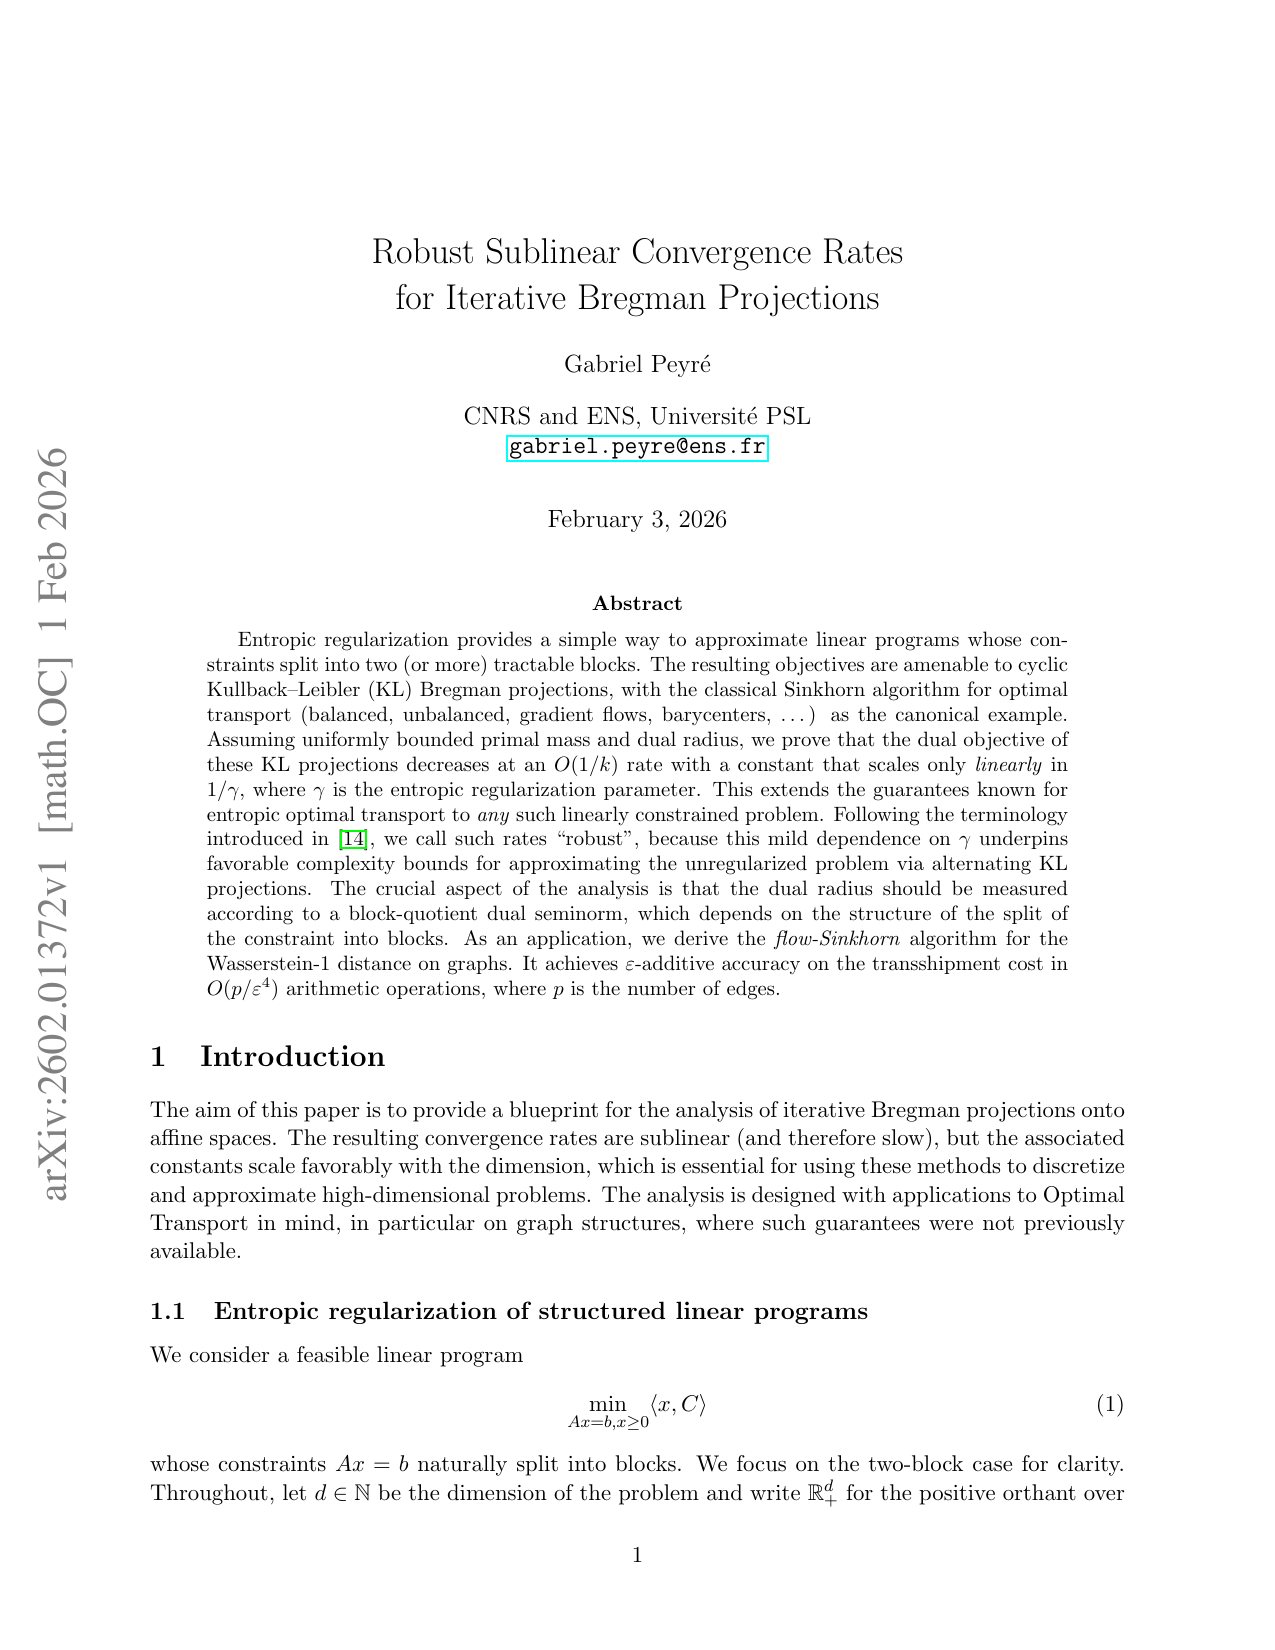
\includegraphics[width=\linewidth,height=0.68\textheight,keepaspectratio]{assets/arxiv_2602_01372_p1.png}
\end{columns}
\source{Retour d'expérience utilisateur + arXiv/GitHub (consulté le 09/03/2026).}
\end{frame}

\begin{frame}{Retour d'expérience d'un groupe}
\begin{columns}[T]
\column{0.55\textwidth}
\scriptsize
\begin{problembox}
\problemlabel{} : évaluation collective au CSD (ENS).
\begin{itemize}
  \keyitem{Protocole}{même prompt, réponses multiples.}
  \keyitem{Tâche}{question semi-ouverte, notebook, code, article, formalisation.}
  \keyitem{Audit}{rendus évalués selon plusieurs critères.}
\end{itemize}
\end{problembox}

\vspace{0.5mm}
\begin{examplebox}
\textbf{Extrait du prompt}\\[-0.3mm]
\tiny\ttfamily
Consider flow matching with a stochastic interpolant a(t)*X0+b(t)*X1.\\
In python/ do an indepth numerical simulation ... X0 sim N(0,Id),\\
X1 is a mixture of three Dirac. In paper/ write a detailed LaTeX article ...\\
compute in closed form Sigma\_t and the flow map T\_t.
\end{examplebox}

\column{0.44\textwidth}
\centering
\fbox{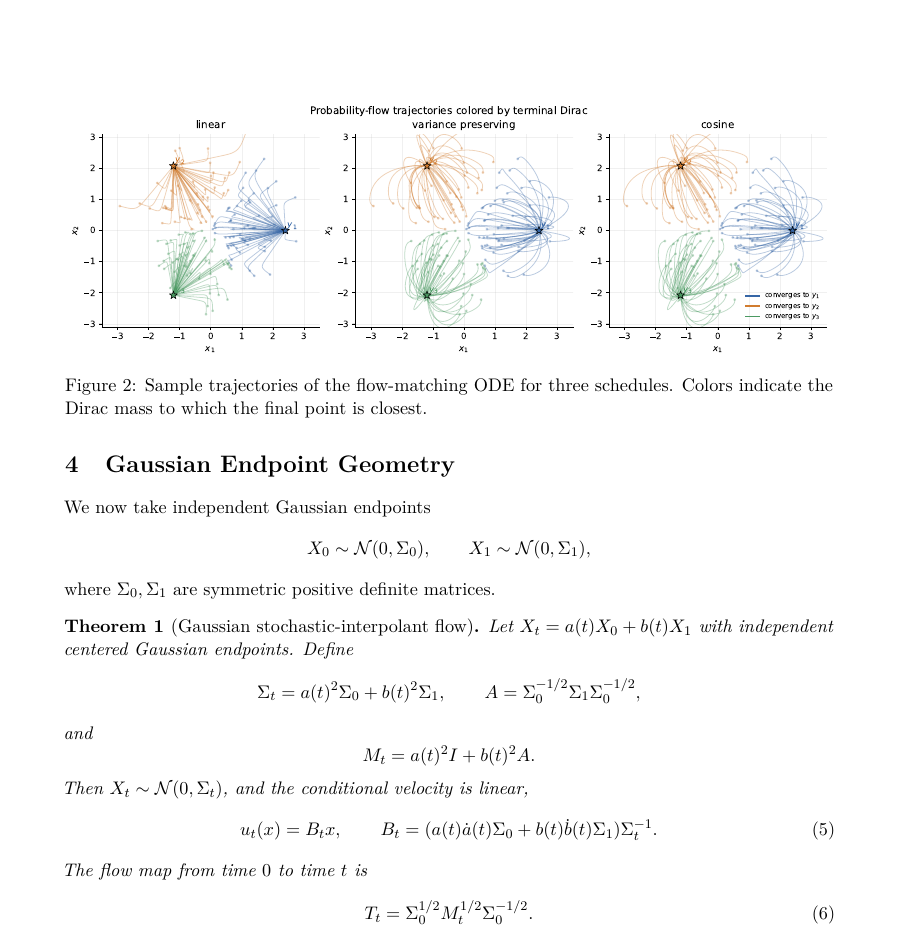
\includegraphics[width=0.90\linewidth,height=0.62\textheight,keepaspectratio]{assets/generated/codex_gabriel_page4_crop.png}}

\vspace{1mm}
\tiny
Snapshot : page d'article issue de la soumission \texttt{codex-gabriel/}.
\end{columns}
\source{ressources/agentic-benchs/todo.md; rapport comparatif du 18/06/2026; soumission codex-gabriel.}
\end{frame}

\begin{frame}{Retour d'expérience d'un groupe (suite)}
\scriptsize
\begin{problembox}
\problemlabel{} : évaluation multicritère.
\end{problembox}

\vspace{0.6mm}
\begin{columns}[T,onlytextwidth]
\column{0.53\textwidth}
\scriptsize
\begin{resultbox}
\resultlabel{} : agrégation par LLM-juge
\vspace{0.3mm}

\centering
\begingroup
\tiny
\setlength{\tabcolsep}{3pt}
\renewcommand{\arraystretch}{0.78}
\begin{tabular}{@{}lccc@{}}
\toprule
Soumission & Maths & Code & Global \\
\midrule
\rowcolor{softTeal}
emmanuel & 9.3 & 8.8 & 9.1 \\
\rowcolor{softTeal}
codex-gabriel & 9.0 & 9.0 & 8.8 \\
openclaw & 8.2 & 8.6 & 8.2 \\
hermes & 7.8 & 8.0 & 7.7 \\
claude-gabriel & 6.5 & 7.5 & 7.1 \\
codex-kimia & 7.0 & 7.0 & 7.0 \\
codex-clement & 7.0 & 5.5 & 6.2 \\
antigravity-a. & 5.8 & 6.0 & 5.8 \\
antigravity-o. & 5.5 & 5.0 & 5.4 \\
\bottomrule
\end{tabular}
\endgroup

\vspace{0.2mm}
\raggedright
\tiny Global = agrégation des critères maths, code, article et robustesse.
\end{resultbox}

\column{0.45\textwidth}
\scriptsize
\begin{resultbox}
\resultlabel{} : signaux robustes
\begin{itemize}
\itemsep0mm
  \keyitem{Maths}{Codex \(\gg\) Claude \(\gg\) reste.}
  \keyitem{Code}{Claude \(\gg\) Codex \(\gg\) reste.}
  \keyitem{Budget}{performance \(\simeq\) tokens.}
\end{itemize}
\end{resultbox}

\vspace{0.1mm}
\begin{takeawaybox}
\takeawaylabel{} : effet du budget tokens
\vspace{0mm}

\tiny
\renewcommand{\arraystretch}{0.82}
\begin{tabular}{@{}p{0.28\linewidth}p{0.64\linewidth}@{}}
\toprule
Budget & Résultat typique \\
\midrule
\rowcolor{softRed}
Petit & preuve incorrecte \\
\rowcolor{softAmber}
Moyen & preuve OK, énoncé perfectible \\
\rowcolor{softTeal}
Gros & solution complète \\
\rowcolor{softGreen}
Énorme & Lean viable \\
\bottomrule
\end{tabular}
\end{takeawaybox}
\end{columns}
\vspace{-2.0mm}
{\tiny\color{aiSlate}Source : Expérience CSD ; audit ressources/agentic-benchs/report.\par}
\end{frame}

\begin{frame}{Zoom : Emmanuel Sérié / Noogram}
\scriptsize
\begin{columns}[T,totalwidth=\linewidth]
\column{0.45\linewidth}
\begin{problembox}
\problemlabel{} : du prompt CSD à un artefact scientifique complet.
\end{problembox}

\vspace{0.6mm}
\begin{resultbox}
\resultlabel{} : contribution Noogram
\begin{itemize}
\itemsep0mm
  \keyitem{Théorème}{FM gaussien \(=\) OT ssi covariances commutent.}
  \keyitem{Artefacts}{site, code, article, figures, Lean, rapport.}
  \keyitem{Audit}{preuve fausse détectée puis corrigée ; score \(\mathbf{9.1}\).}
\end{itemize}
\end{resultbox}

\vspace{0.6mm}
\begin{takeawaybox}
\takeawaylabel{} : harnessing d'agents pour la science.
\begin{itemize}
\itemsep0mm
  \keyitem{Chaîne}{générer, tester, réfuter, publier.}
  \keyitem{Rigueur}{ancrage par un expert Lean.}
  \keyitem{Coût}{lourd, mais auditable de bout en bout.}
\end{itemize}
\end{takeawaybox}

\column{0.53\linewidth}
\centering
\fbox{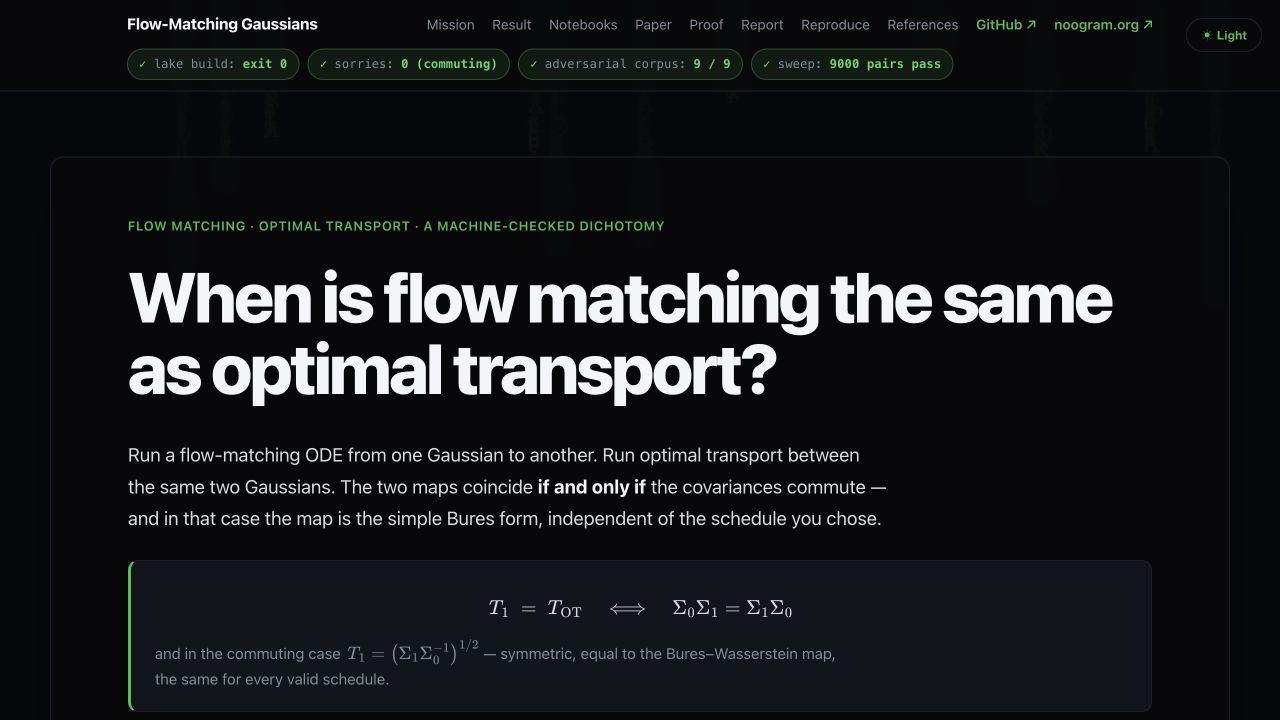
\includegraphics[width=0.98\linewidth,height=0.31\textheight,keepaspectratio]{assets/generated/noogram_flow_matching_site.png}}

\vspace{0.8mm}
\fbox{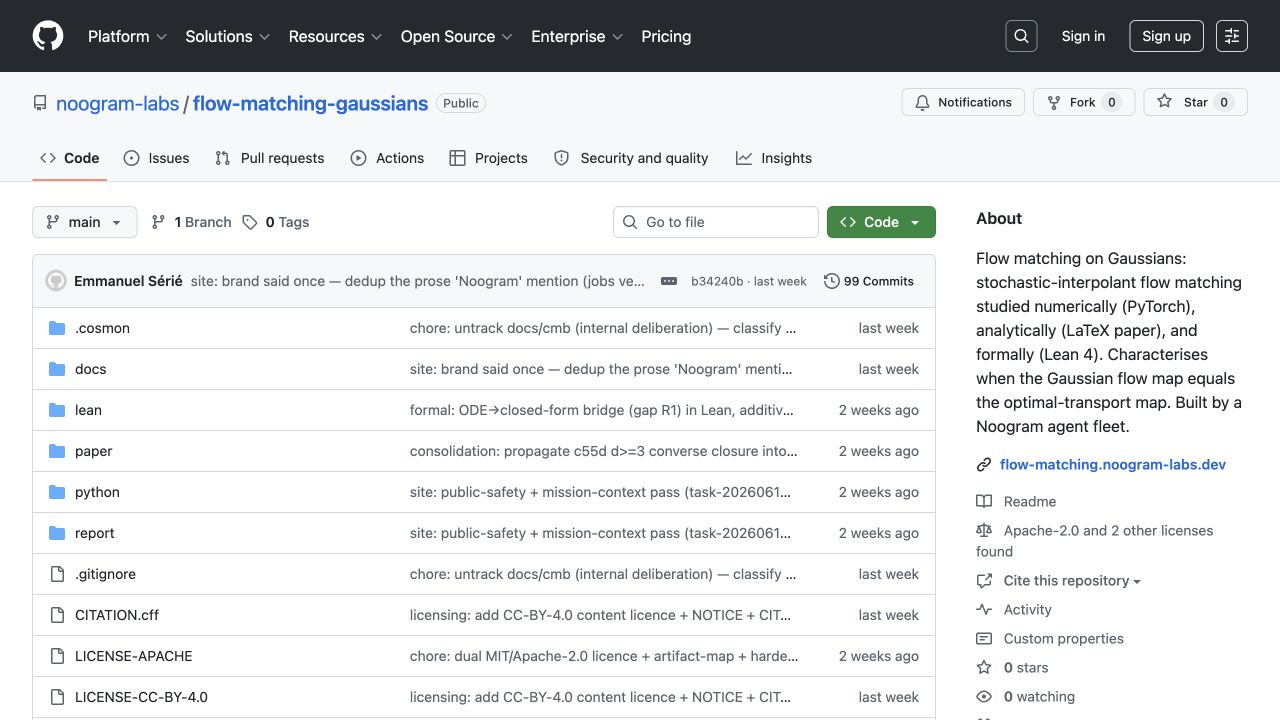
\includegraphics[width=0.98\linewidth,height=0.27\textheight,keepaspectratio]{assets/generated/noogram_flow_matching_github.png}}

\vspace{0.4mm}
{\tiny\color{aiSlate}\raggedright Sources : site Noogram ; GitHub \texttt{noogram-labs/flow-matching-gaussians} ; audit CSD.\par}
\end{columns}
\end{frame}

\planslide{4}

\begin{frame}{Impact sur l'évaluation et l'enseignement}
\small
\begin{minipage}[t]{0.48\linewidth}
\vspace{0pt}
\begin{neutralboxalt}
\textbf{Reviewing} : l'IA comme premier lecteur
\vspace{0.6mm}

\centering
\fbox{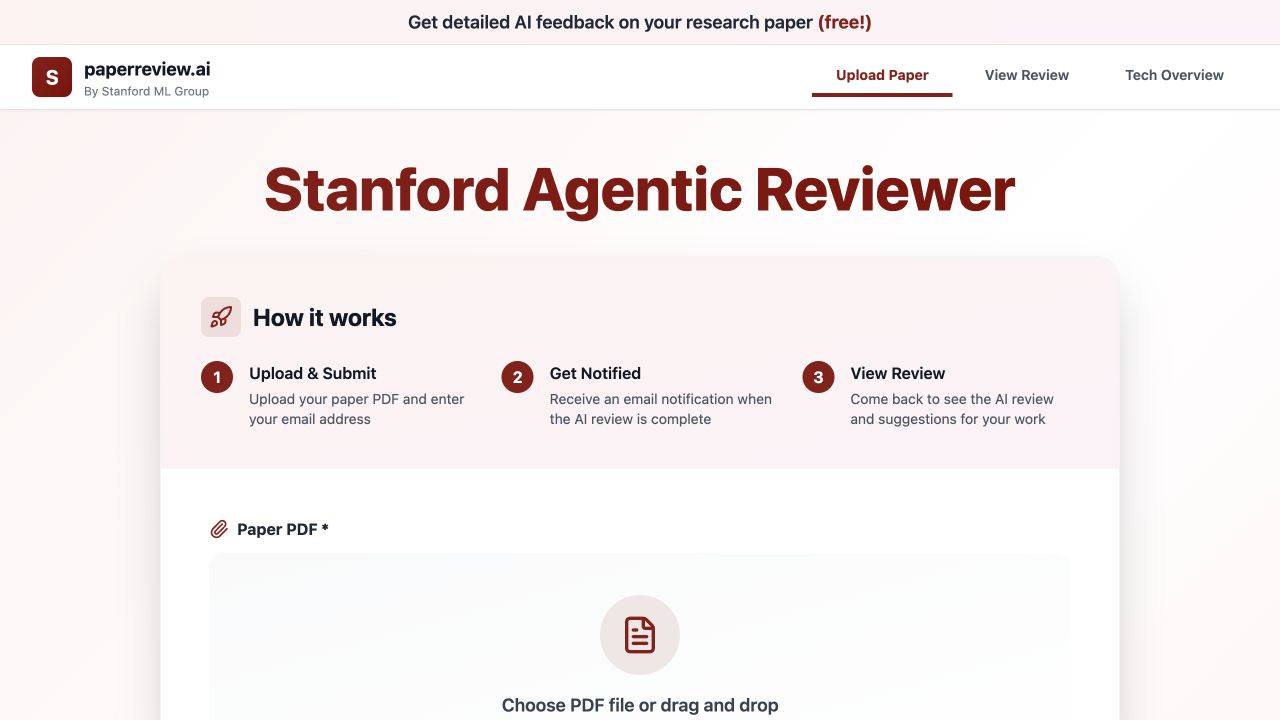
\includegraphics[width=0.93\linewidth,height=0.31\textheight,keepaspectratio]{assets/generated/paperreview_ai_screenshot.png}}

\vspace{0.6mm}
\raggedright
\scriptsize
\begin{itemize}
\itemsep0mm
  \keyitem{Automatisation}{premier rapport, failles locales, suggestions.}
  \keyitem{Signal faible}{triage, pas validation scientifique.}
  \keyitem{Valeur humaine}{validité, nouveauté, goût.}
\end{itemize}
\end{neutralboxalt}
\end{minipage}\hfill
\begin{minipage}[t]{0.48\linewidth}
\vspace{0pt}

\begin{neutralbox}
\textbf{Enseignement} : préserver la formation humaine
\vspace{0.5mm}

\scriptsize
\begin{itemize}
\itemsep0.4mm
  \keyitem{Niveau}{doctorant pour rédaction, code, critique.}
  \keyitem{Risque}{déléguer avant d'avoir appris à raisonner.}
  \keyitem{Perte}{futurs enseignants, rapporteurs, évaluateurs d'IA.}
  \keyitem{À protéger}{oral, critique de preuves, audit d'IA.}
\end{itemize}
\end{neutralbox}
\end{minipage}
\source{\href{https://paperreview.ai/}{PaperReview.ai}, Stanford ML Group (capture 02/07/2026) ; synthèse qualitative.}
\end{frame}

\begin{frame}{Actions pour la communauté}
\footnotesize
\begin{columns}[T,totalwidth=\linewidth]
\column{0.49\linewidth}
\begin{actionbox}
\begin{columns}[T,totalwidth=\linewidth]
\column{0.62\linewidth}
\textbf{Structurer la communauté}
\column{0.34\linewidth}
\vspace{-1.4mm}
\centering

\includegraphics[width=\linewidth,height=0.10\textheight,keepaspectratio]{assets/generated/aissai_logo.png}
\end{columns}
\vspace{-1.2mm}
\begin{itemize}
\itemsep0mm
  \keyitem{CNRS RT}{pont IA, maths, formalisation, CS (INSMI/INS2I).}
  \keyitem{AISSAI}{trimestre « IA pour les maths » couplé au RT.}
\end{itemize}
\end{actionbox}

\vspace{1.4mm}
\begin{claimbox}
\textbf{Ouvrir l'accès aux modèles}
\begin{itemize}
  \keyitem{Dépôts}{projets académiques reliés aux modèles.}
  \keyitem{Modèles}{contrôle et auditabilité.}
\end{itemize}
\end{claimbox}

\column{0.49\linewidth}
\begin{examplebox}
\textbf{Dialogue avec l'industrie}
\begin{itemize}
  \keyitem{DeepMind}{finance programme postdoc AISSAI.}
  \keyitem{Mistral}{outils Emmy pour le CNRS à faire évoluer.}
\end{itemize}
\end{examplebox}

\vspace{1.4mm}
\begin{riskbox}
\textbf{Ne pas oublier la formation}
\begin{itemize}
  \keyitem{Professeurs}{conception + évaluation.}
  \keyitem{Évaluateurs}{formation humaine préservée.}
\end{itemize}
\end{riskbox}
\end{columns}
\end{frame}

\begin{frame}{Conclusion}
\footnotesize
\begin{columns}[T,totalwidth=\linewidth]
\column{0.49\linewidth}
\begin{claimbox}
\textbf{1. Accélération déjà visible}
\begin{itemize}
  \keyitem{Performance}{progrès \textbf{très rapides} en maths.}
  \keyitem{Workflows}{coder, vérifier, rédiger.}
\end{itemize}
\end{claimbox}

\vspace{1.4mm}
\begin{proofbox}
\textbf{2. Impact scientifique concret}
\begin{itemize}
  \keyitem{Informel}{problèmes ouverts débloqués.}
  \keyitem{Formel}{Lean en progrès, coût tokens élevé.}
\end{itemize}
\end{proofbox}

\column{0.49\linewidth}
\begin{examplebox}
\textbf{3. Rôle humain déplacé}
\begin{itemize}
  \keyitem{Positionnement}{augmenter, pas remplacer.}
  \keyitem{Rôle}{chercheur \(\rightarrow\) juge de qualité des preuves.}
\end{itemize}
\end{examplebox}

\vspace{1.4mm}
\begin{riskbox}
\textbf{4. Enjeux collectifs}
\begin{itemize}
  \keyitem{Accès}{modèles contrôlables et auditables.}
  \keyitem{Tension}{échanges académie--industrie.}
  \keyitem{Souveraineté}{cadre scientifique public.}
\end{itemize}
\end{riskbox}
\end{columns}
\end{frame}

\end{document}
